%% appendix/within-class-study.tex
%% Appendix: spikes within a single class (small-data study).
%% Register: Genzer -- parsimonious, direct, no hyperbole. No em dashes, US spelling.
%% Cross-references the clustering section rather than re-deriving it; the new
%% content is the within-class experiment and the eigengap-versus-bulk-edge
%% lesson for counting spikes on real data. Figure from notebooks/05.

\section{Spikes Within a Single Class}\label{app:within-class}

Section~\ref{sec:clustering} reads classes off spikes: well-separated groups leave isolated outliers above the bulk of the Gram matrix \(\mat{G} = \frac{1}{p}\mat{X}\transpose\mat{X}\), and its leading eigenvectors estimate the labels. Two questions are natural once the method is in hand. What does the same procedure report inside a single class, where there is no between-class signal? And how should the number of spikes be read on real data, where the Gaussian model of Section~\ref{subsec:clustering} no longer holds exactly? This appendix records a small study of both on the MNIST digits.

\paragraph{One digit is one class.} Running the pipeline on the images of a single digit, with no labels and the common mean shape removed first as in Section~\ref{subsec:mnist}, produces no fundamental spike. For the \(0\) and, separately, for the more variable \(7\), the spectrum of \(\mat{G}\) carries no isolated outlier: the leading eigenvalues decay smoothly into the bulk, the top eigenvector varies continuously across the points rather than splitting into levels, and the embedding is a single cloud (Figure~\ref{fig:within-class}, top, for the \(0\)). A genuine sub-class, one whose signal-to-noise ratio cleared the threshold of Theorem~\ref{thm:gram-spikes}, would split the eigenvector entries into two levels, one per group, each blurred into a Gaussian by Theorem~\ref{thm:eigvec-clt}; with no such sub-class the entries form a single noisy band. The directions along which a digit does vary, such as slant, stroke width and size, are continuous rather than discrete, and forcing two clusters returns near-identical averages. The control confirms the contrast. Placing the same images flush left or shifted a few pixels to the right injects a real difference in means; one eigenvalue then separates well above the bulk, the embedding splits in two, and the sign of the top eigenvector recovers the partition (Figure~\ref{fig:within-class}, bottom). A single digit offers no second mean to separate, so its sub-class signal-to-noise ratio is zero and, by Theorem~\ref{thm:gram-spikes}, no spike can appear.

\begin{figure}[H]
  \centering
  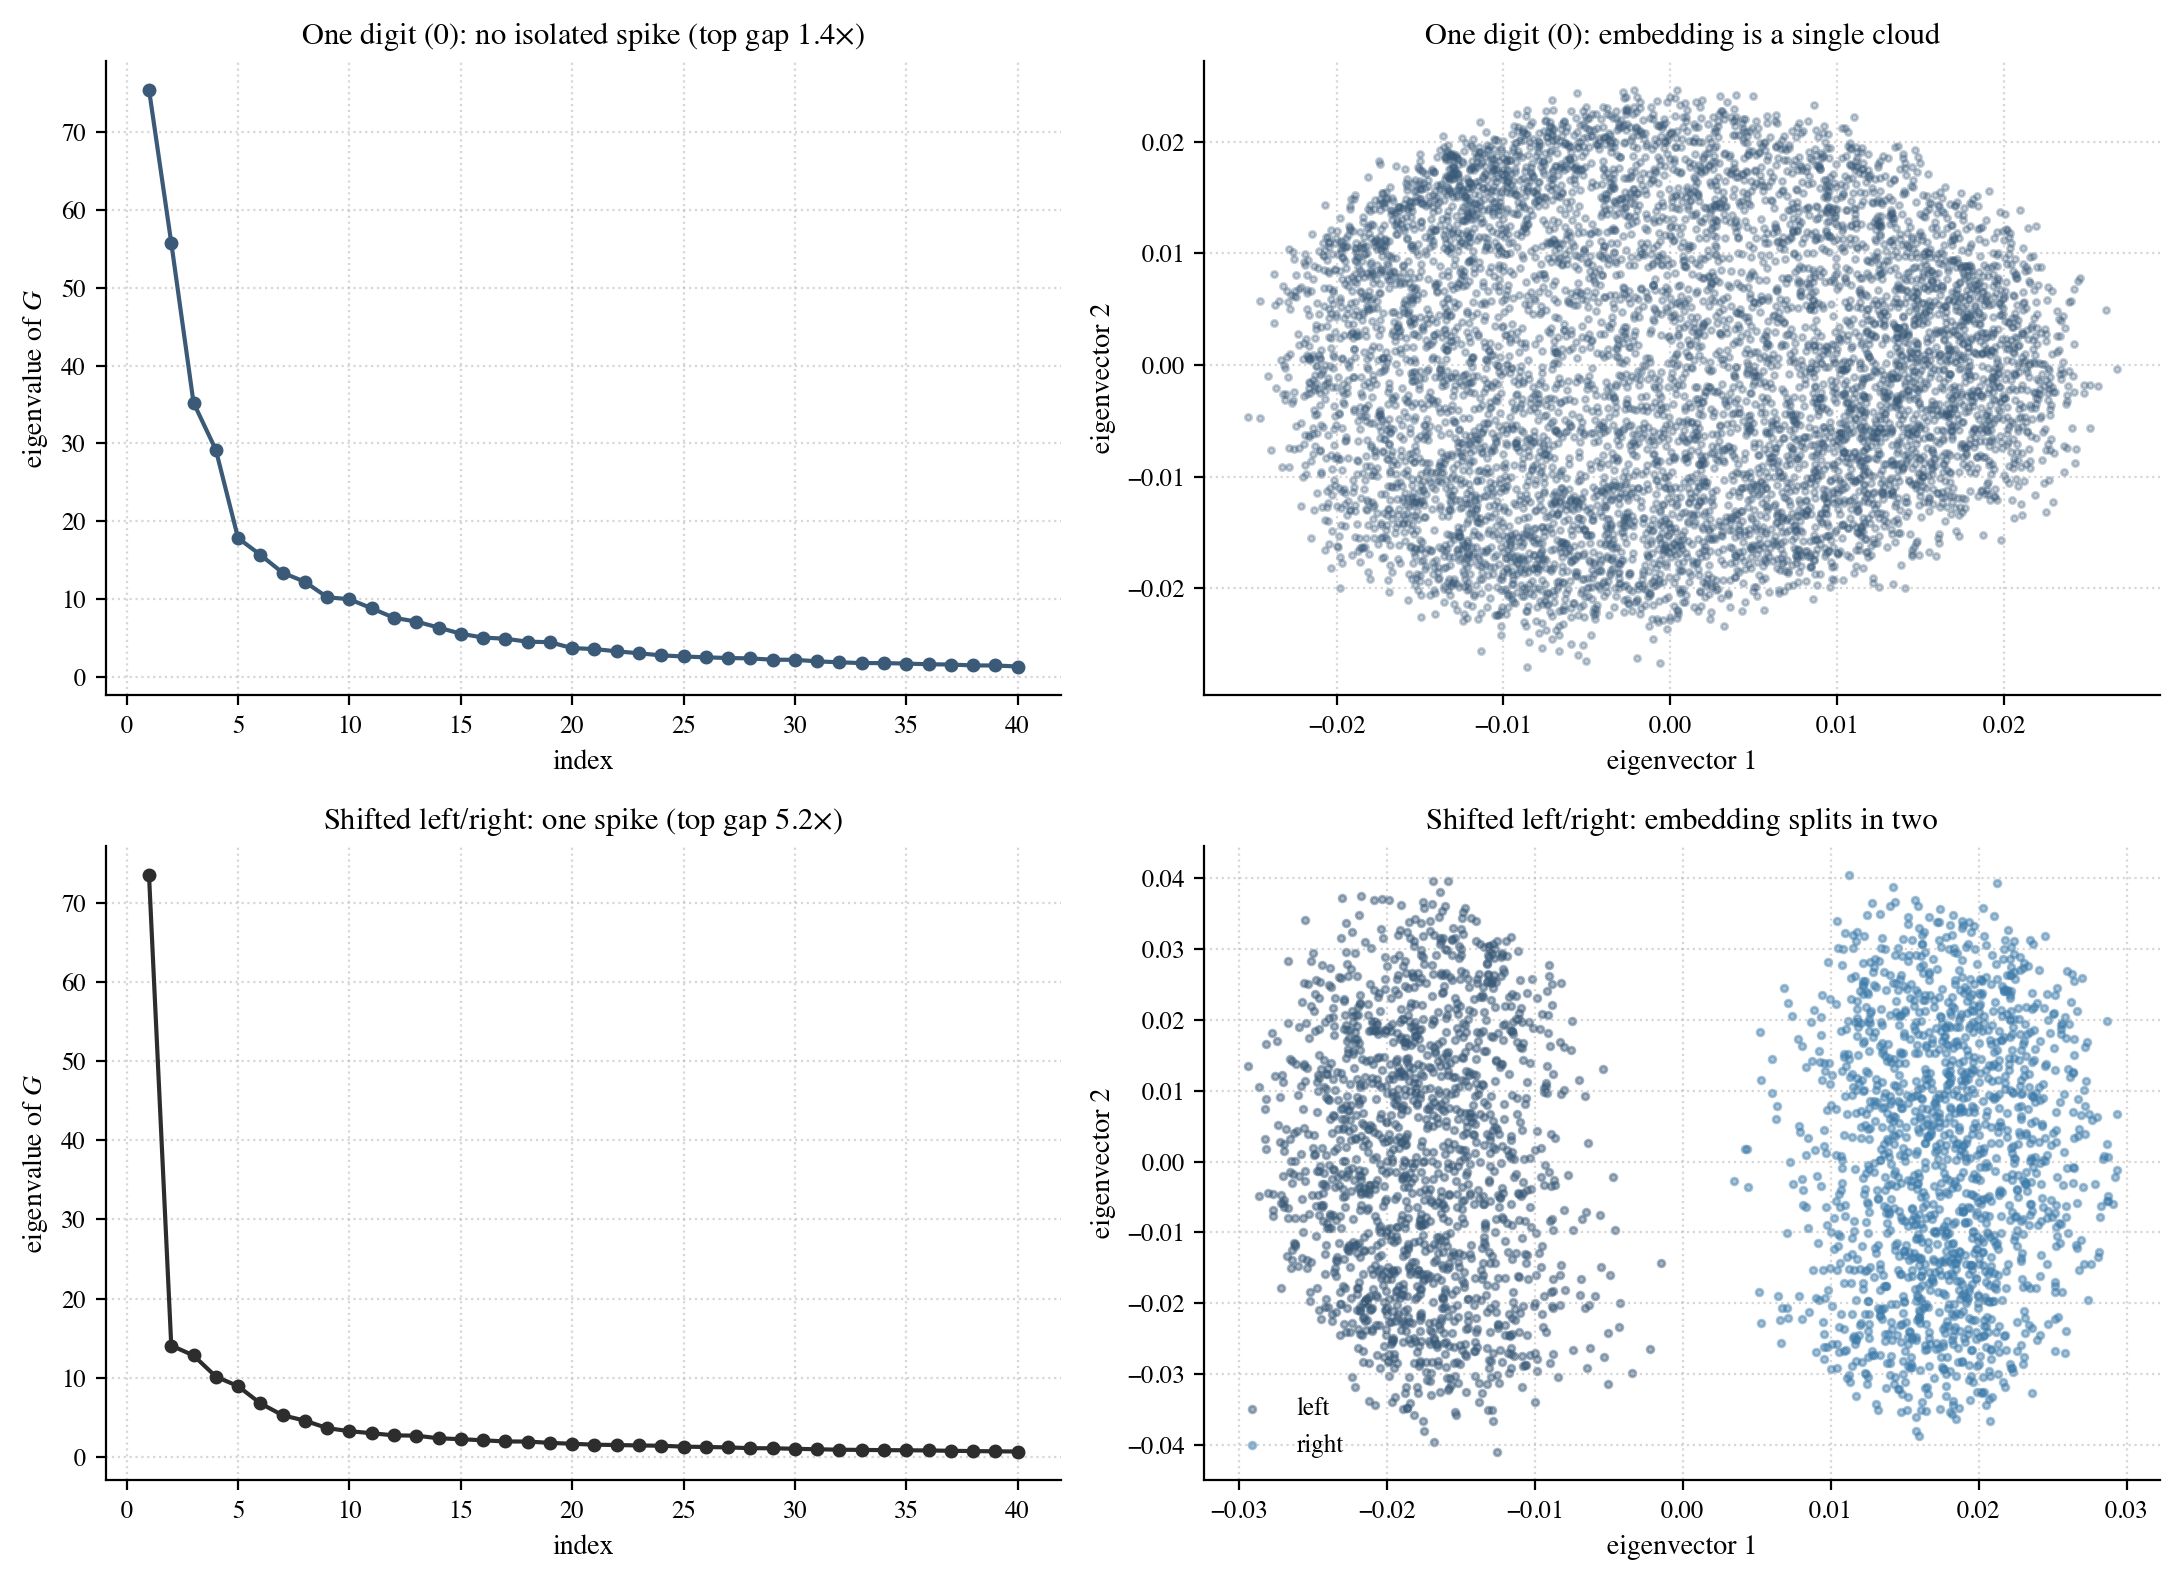
\includegraphics[width=0.95\textwidth]{figures/within_class_study.png}
  \caption{Spikes within a single class versus an injected two-class structure (MNIST; no labels are used, and the common mean image is removed first). \emph{Top:} the digit \(0\) on its own. The eigenvalues of \(\mat{G}\) decay smoothly with no isolated outlier (the largest is only \(1.4\) times the next), and the two-dimensional embedding is a single cloud, so the leading eigenvectors point to one class. \emph{Bottom:} the same images placed flush left or shifted eight pixels to the right, a genuine two-class structure. One eigenvalue now separates well above the bulk (the largest is \(5.2\) times the next) and the embedding splits cleanly, recovered by the sign of the top eigenvector. Generated by \texttt{notebooks/05\_clustering\_demos.py}.}
  \label{fig:within-class}
\end{figure}

\paragraph{Counting spikes on real data.} The study also corrected a tempting recipe. In the white-noise model of Theorem~\ref{thm:gram-spikes} a fundamental spike is an eigenvalue above the bulk edge \((1 + 1/\sqrt{y})^2\), with everything else collapsing into the bulk; but that edge is located only when the noise is white with a known variance \(\sigma^2\), where it sits at \(\sigma^2(1 + 1/\sqrt{y})^2\). Real images are not white noise. Their within-class variation is correlated and concentrated on a low-dimensional set, so most sample eigenvalues lie near zero and there is no flat noise floor from which to estimate \(\sigma^2\); a plug-in edge then collapses toward zero and would count hundreds of continuous-variation directions as spikes, even for a single digit. The robust signature is instead \emph{isolation}. A fundamental spike is an eigenvalue separated from the bulk by a clear gap, the eigengap heuristic of \citet{vonLuxburg2007}; equivalently, by Theorem~\ref{thm:eigvec-clt}, its eigenvector splits the points into levels rather than forming one noisy band. Isolation needs no noise model, and it is the criterion we use to count classes here.

\clearpage
